% /Users/philchodrow/.../main.tex
% RevTeX 4.2 minimal starter document

\documentclass[aps,pre,reprint,superscriptaddress,nofootinbib]{revtex4-2}

\usepackage{amsmath,amssymb,bm}
\usepackage{graphicx}
\usepackage{hyperref}
\hypersetup{colorlinks=true,linkcolor=blue,citecolor=blue,urlcolor=blue}

\input{macros}

\begin{document}

\title{Growing Hypergraphs with Node Labels}
\author{Francis Cataldo$^*$}
\affiliation{Department of Computer Science, Middlebury College, Middlebury, VT, USA}
\author{Violet Ross$^*$}
\affiliation{Department of Computer Science, University of Colorado at Boulder, Boulder, CO, USA}
\author{Philip S. Chodrow}
\affiliation{Department of Computer Science, Middlebury College, Middlebury, VT, USA}


\date{\today}
\begin{abstract}
    We study a generative mechanistic model of hypergraph growth in which nodes possess binary labels which generalizes prior work on edge-copying growing hypergraphs.  
    Edges form in this model as noisy copies of previous edges, where the transmission of nodes from one edge to the next depends on the labels. 
    We derive a power law for the degree distribution in this model and describe the long-term dynamics of the joint distribution of labels contained in edges. 
    We then demonstrate that this model can be learned from data: we can both estimate the parameters of the model via (stochastic) expectation maximzation and perform community detection of the node labels via maximum-likelihood estimation. 
\end{abstract}

\maketitle

\def\thefootnote{*}\footnotetext{Equal author contributions}\def\thefootnote{\arabic{footnote}}


% \def\thefootnote{*}\footnotetext{These authors contributed equally to this work}\def\thefootnote{\arabic{footnote}}


\section{Introduction}

\section{Long-Run Dynamics}

\phil{What's in here is mostly notes and needs to be cleaned up some.}

\subsection{Mean Degree}

The mean degree $\brackets{d}$ of a node satisfies 
\begin{align}
    \brackets{d} = \frac{m}{n}\brackets{k} \;,
\end{align}
where $\brackets{k}$ is the mean edge size, $m$ is the number of edges, and $n$ is the number of nodes.
In expectation, there are $\gamma_- + \gamma_+$ new nodes added per new edge, which means that $\frac{m}{n} \to \frac{1}{\gamma_- + \gamma_+}$ as $m, n \to \infty$ in expectation.
So, we have 
\begin{align}
    \brackets{d} = \frac{\brackets{k}}{\gamma_- + \gamma_+} \;.
\end{align}
We don't have a closed-form expression for the stationary value of $\brackets{k}$, but we can compute it numerically from the stationary distribution of the joint label counts $p(k_0, k_1)$. 






\subsection{Power Law Degree Distribution}




This argument follows that of \cite{heEdgeCorrelationsLink2025}, which in turn is based on a derivation by \cite{mitzenmacherBriefHistoryGenerative2004}. 

Under the mean-field assumption that the degree of a node is independent of the ratio $\frac{k_0}{k}$ of the edge it is contained in, we can write down an argument to show that the degree distribution follows a power law and give a formula for the exponent. 
Define the moments 
\begin{align}
    \rho_{0} &= \brackets{\frac{k_0^2}{k}} \quad \text{,} \quad \rho_{1} &= \brackets{\frac{k_1^2}{k}} \quad \text{and} \quad \rho_{01} = \brackets{\frac{k_0 k_1}{k}} \;.
\end{align}
Then, the expected number of nodes which are sampled in the edge-sampling step is 
\begin{align}
    \sigma \triangleq 1 + \eta_+ \squarebrackets{\rho_0 + \rho_1 - 1} + \eta_- \rho_{01}\;.
\end{align}
Importantly, $\sigma$ depends only on the parameters and the moments of the joint distribution $p(k_0, k_1)$, which we are going to show how to get from linear algebra later.
Let $\tilde{\sigma} = \frac{\sigma}{\brackets{d}}$, where $\brackets{d}$ is the average degree of a node in the hypergraph.

Under a mean-field assumption in which the degree $d$ of a node is independent from the counts $k_0$ and $k_1$ of labels in an edge containing that node, we can give the expected change in the count of degree $d$ nodes as 
\begin{align}
    \tilde{\sigma} ((d-1)p_{d-1}^{(t)} - d p_d^{(t)})
\end{align}
Similarly, the expected number of nodes which are sampled in the extant node addition step is $\lambda_+ + \lambda_-$. 
This gives, in expectation for the change in degree $d$ nodes, 
\begin{widetext}
    \begin{align}
        n^{(t+1)}p_{d}^{(t+1)} - n^{(t)}p_{d}^{(t)} = \tilde{\sigma} \squarebrackets{(d-1)p_{d-1}^{(t)} - d p_d^{(t)}} + (\lambda_+ + \lambda_-) (p_{d-1}^{(t)} - p_d^{(t)}) \;.
    \end{align}
\end{widetext}
We know that at stationarity, $n^{(t+1)} - n^{(t)}$ is in expectation equal to $\gamma_+ + \gamma_-$, while at stationarity $p_d^{(t+1)} = p_d^{(t)} = p_d$. 
Thus, we obtain 
\begin{widetext}
    \begin{align}
        p_d \paren{\gamma_+ + \gamma_-}  = \tilde{\sigma} \squarebrackets{(d-1)p_{d-1} - d p_d} + (\lambda_+ + \lambda_-) (p_{d-1} - p_d) \;.
    \end{align}
\end{widetext}
Rearranging, we obtain 
\begin{align}
    \frac{p_d}{p_{d-1}} &= \frac{\tilde{\sigma}(d-1) + \lambda_+ + \lambda_-}{\tilde{\sigma} d + \gamma_+ + \gamma_- + \lambda_+ + \lambda_-} \\ 
    &= 1 - \frac{\tilde{\sigma} + \gamma_+ + \gamma_-}{\tilde{\sigma} d + \gamma_+ + \gamma_- + \lambda_+ + \lambda_-}
\end{align}
Allowing $d$ to become large (which describes the tail of the degree distribution), we have
\begin{align}
    \frac{p_d}{p_{d-1}} &\approx 1 - \frac{\tilde{\sigma} + \gamma_+ + \gamma_-}{\tilde{\sigma} d} \;,
\end{align}
a relation which corresponds to a power law with exponent $\zeta = 1 + \frac{\gamma_+ + \gamma_0}{\tilde{\sigma}}$. 
Explicitly calculating this moment requires computing the moments $\rho_0$, $\rho_1$, and $\rho_{01}$, which can be done computationally from the stationary joint distribution $p(k_0, k_1)$. 

\subsection{Joint Distribution of Labels}


\begin{figure*}[t]
    \centering
    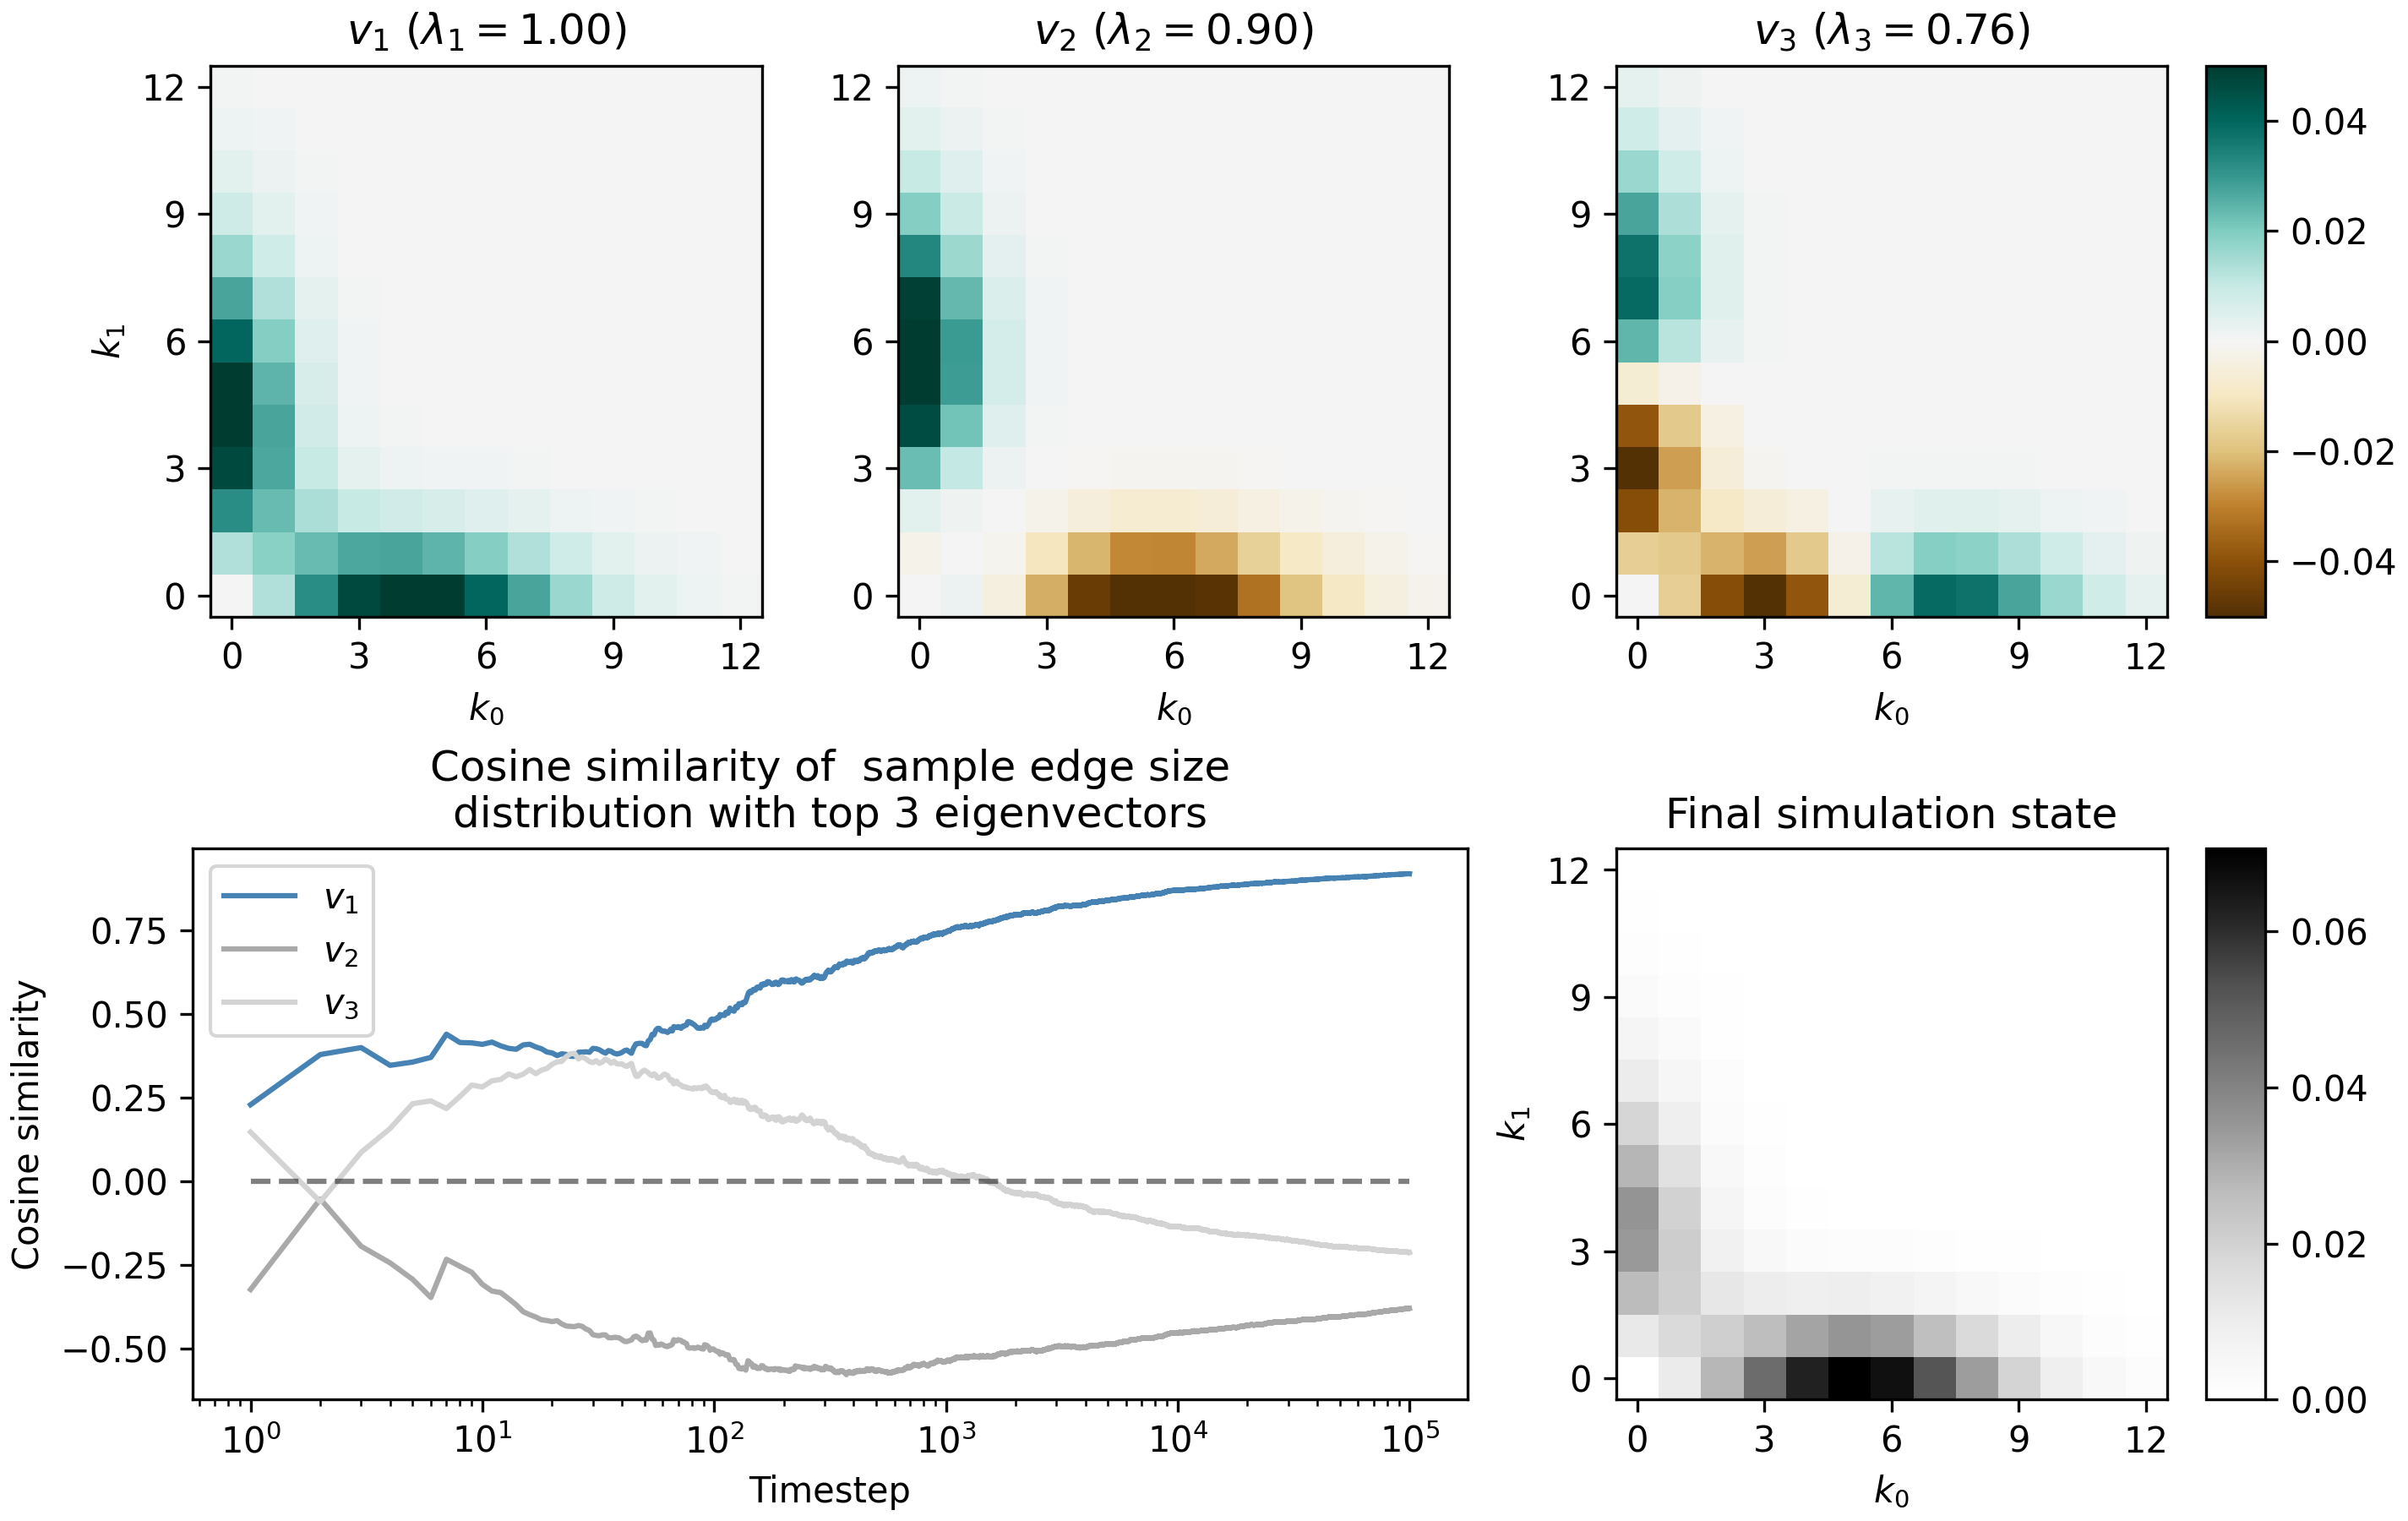
\includegraphics[width=1\textwidth]{../fig/linear_map_eigenvectors.png}
    \caption{Dynamics! Top shows the three leading eigenvectors of the distribution $p(k_0, k_1)$. Bottom left gives the cosine similarity (normalized projection) between one run of simulation dynamics and these eigenvectors. Bottom right gives the efinal simulation state.}
    \label{fig:example}
\end{figure*}


\section{Model Inference}

\phil{Someone needs to establish standardized notation in this section. }

\subsection{Parameter Estimation via Stochastic EM}

\phil{Violet, this is your spot! Descriptions of methods/algorithms should go here, results are for later. }


\subsection{Community Detection via MLE}

\phil{Frannie, this is your spot! Descriptions of methods/algorithms should go here, results are for later.}


\section{Inference Results}

How did we do on real and synthetic data? 




\section{Conclusion}
Blah blah blah. 

\begin{acknowledgments}
PSC acknowledges support from the National Science Foundation under DMS-2407058.
\end{acknowledgments}

\bibliographystyle{apsrev4-2}
\bibliography{refs} 

\end{document}

